\documentclass[acmsmall,review,nonacm]{acmart}
\usepackage{pdfpages}
\usepackage{booktabs}
\usepackage{longtable}
\usepackage{array}
\usepackage{tabularx}
\usepackage{enumitem}
\usepackage{tikz}
\usetikzlibrary{arrows.meta,positioning,patterns,calc}
\usepackage{microtype}
\settopmatter{printacmref=false,printfolios=true}
\setcopyright{none}
\acmJournal{TOPLAS}
\acmSubmissionID{}
\title[Observation-Stable Model Unweaving]{Observation-Stable Model Unweaving: Local Certificates and a Two-Write Boundary}
\author{Haoyi Zhang}
\affiliation{\institution{Xi'an Jiaotong-Liverpool University}\city{Suzhou}\country{China}}
\email{hyeliozhang@gmail.com}
\author{Huaijin Ran}
\affiliation{\institution{Nanyang Technological University}\city{Singapore}\country{Singapore}}
\email{huaijin003@e.ntu.edu.sg}
\renewcommand{\shortauthors}{Zhang and Ran}
\hypersetup{pdftitle={Observation-Stable Model Unweaving: Local Certificates and a Two-Write Boundary},pdfauthor={Haoyi Zhang and Huaijin Ran}}
\begin{document}
% The inherited 35-page body was supplied only as a compiled PDF.  Pages 1--33
% are preserved exactly; its two-page bibliography is replaced by the unified
% bibliography below.  Editable proof, evidence, and calibration additions begin
% on page 34.  This assembly decision is documented in CURRENT-STATE.md.
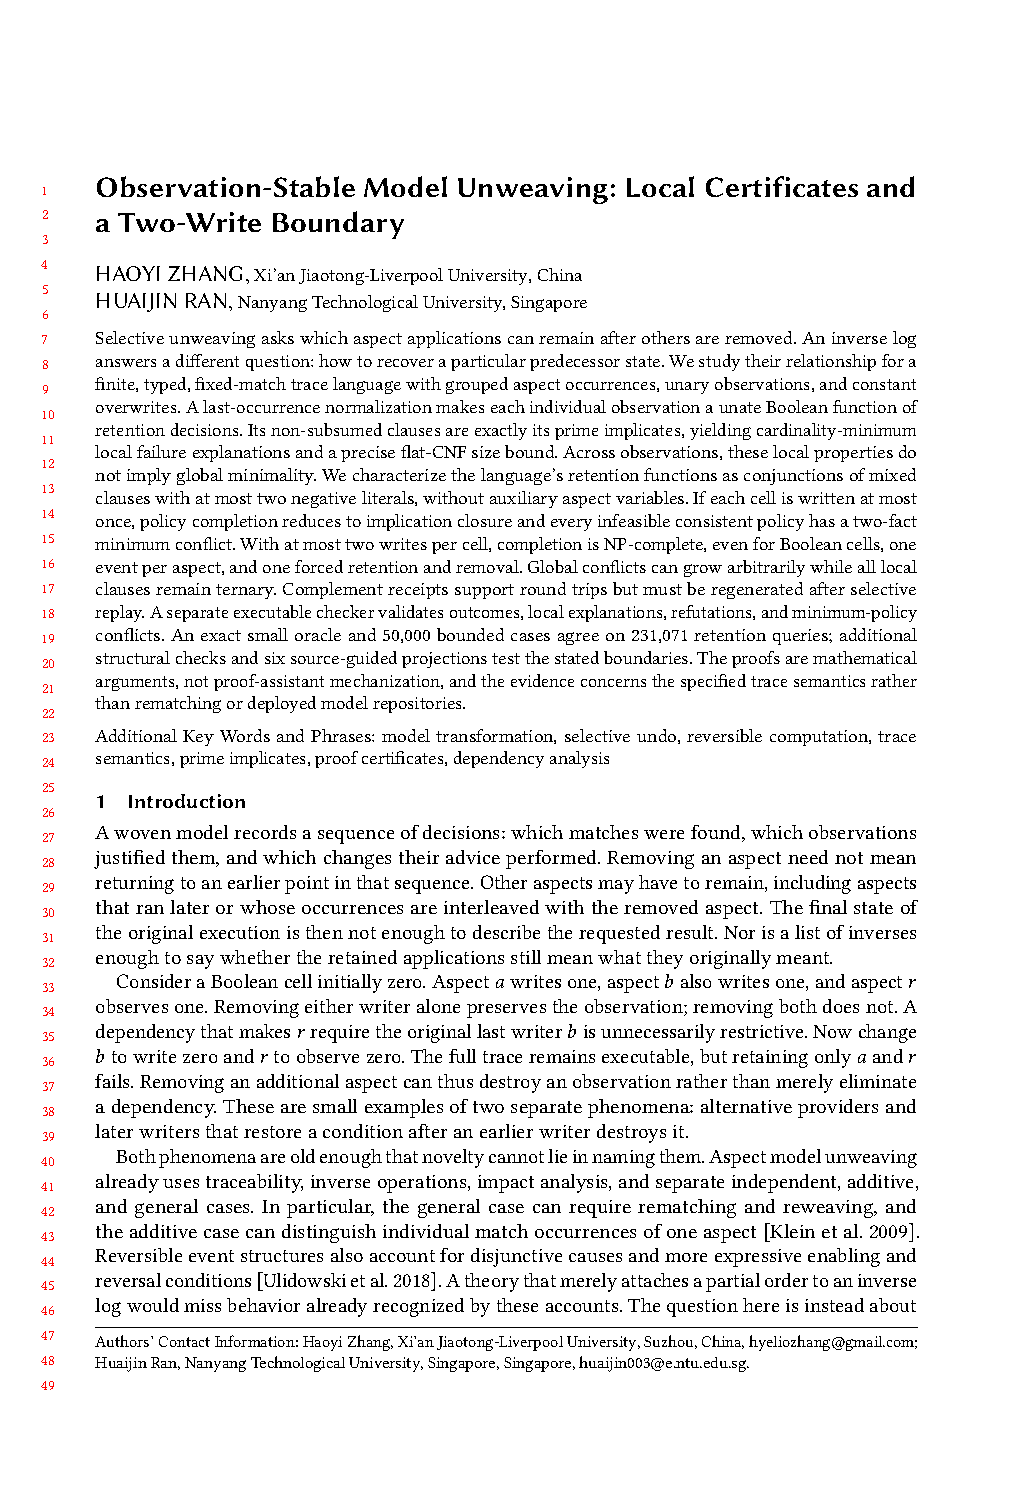
\includepdf[pages=1-33,fitpaper=true,pagecommand={\thispagestyle{empty}}]{frozen-body.pdf}
\setcounter{page}{34}
\appendix
\section{Proof Architecture and Evidence Qualification}
\label{app:proofs}

This appendix makes the proof and evidence boundary explicit in a form that can be
checked without reading implementation identifiers into the semantic argument.  The
main text uses ordinary theorem prose.  The standalone repository additionally
numbers the corresponding proof obligations T1--T26 so that a checker result, a raw
record, and a manuscript claim can be joined without pretending that finite execution
is a proof assistant.  The central interface is deliberately small: a finite catalog
of typed cells, a fixed and already executable sequence of captured events, unary
observations, simultaneous constant overwrites, and one retention bit per aspect tag.
All occurrences of a tag are retained or erased together and retained occurrences keep
their original order.  No theorem below quantifies over rematching, fresh identity
generation, arbitrary imperative advice, hidden side effects, or semantic equivalence
between unrelated models.

\subsection{Semantic objects and judgments}

A signature is a tuple
$\Sigma=(X,(D_x)_{x\in X},N,E,s,t)$, where $X$ is a finite set of
cells, every $D_x$ is finite and nonempty, $N,E\subseteq X$ are disjoint
Boolean node and edge-presence cells, and each $e\in E$ has fixed endpoints
$s(e),t(e)\in N$.  A state $\sigma$ maps every cell to a value in its domain.
It is well typed when
\[
  \forall e\in E.\quad \sigma(e)=1\Longrightarrow
       \sigma(s(e))=\sigma(t(e))=1.
\]
An event occurrence is $e_i=(a_i,g_i,w_i)$: $a_i$ is an aspect tag,
$g_i$ maps finitely many cells to nonempty accepting subsets of their domains,
and $w_i$ is a finite map of cells to constants.  Enabled execution is
\[
 \sigma \xrightarrow{e_i} \tau
 \quad\Longleftrightarrow\quad
 \bigl(\forall x\in\mathrm{dom}(g_i).\ \sigma(x)\in g_i(x)\bigr)
 \land \tau=\sigma[w_i].
\]
The original trace $T=e_0\cdots e_{n-1}$ must execute from a well-typed base
$B$.  A retention set $K$ contains tags, not occurrences.  The selected trace
$T\!
estriction K$ contains exactly the occurrences whose tags lie in $K$,
in original order.  Its replay is \emph{observation stable} when every retained
occurrence is enabled at the selected predecessor generated by that replay.

The typing rule is intentionally sufficient rather than complete.  For every edge
and endpoint pair changed by an event, the rule requires the post-edge to be
certainly absent or the post-endpoint to be certainly present.  A written constant
establishes certainty directly; an unchanged cell can establish it through a
singleton observation.  The rule admits simultaneous deletion of an edge and an
endpoint and proves forward preservation by an incidence-by-incidence case split.
It does not infer all consequences of graph typing, and therefore no completeness
claim is attached to it.

For a written coordinate $x$, define its possible pre-value set
$A_i(x)=g_i(x)$ when observed and $A_i(x)=D_x$ otherwise.  A receipt stores the
actual old value exactly when $|A_i(x)|>1$ and identifies the occurrence whose
write it reverses.  The inverse checks the written post-values, restores each
coordinate from either the receipt or the unique member of $A_i(x)$, and rechecks
the event observations.  This yields one-step and trace round trips.  In the scalar
product fragment, omitting any non-singleton overwritten coordinate identifies two
enabled pre-states with the same post-state and stored coordinates, proving the
coordinate-level necessity result.  The result is not a minimum-bit encoding theorem
and does not apply when relational invariants infer omitted values.

Selective replay changes the predecessor of a retained occurrence.  For example,
from base $x=0$, aspect $a$ writes $1$ and aspect $b$ writes $2$.  The original
receipt for $b$ stores $1$, whereas the selected execution that retains only $b$
requires a receipt storing $0$.  Thus an executable selected trace and a correct
selected final state do not justify reusing an old complement.  The regenerated
receipt, not the original one, is the witness checked by a successful outcome
certificate.  Figure~\ref{fig:rebasing-app} restates this boundary using the
reconstructed editable figure source delivered with the project.

\begin{figure}[t]
  \centering
  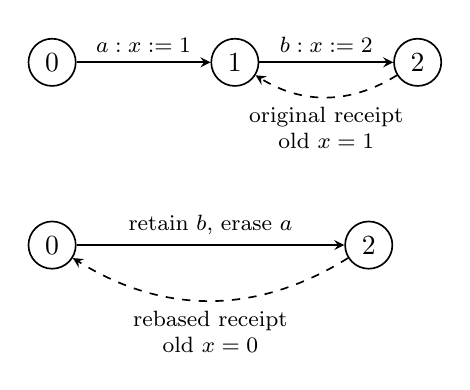
\begin{tikzpicture}[>=stealth,semithick,node distance=14mm and 17mm,
 state/.style={draw,circle,minimum size=6mm,inner sep=1pt},
 lab/.style={font=\footnotesize,align=center}]
\node[state] (s0) {$0$};
\node[state,right=of s0] (s1) {$1$};
\node[state,right=of s1] (s2) {$2$};
\draw[->] (s0) -- node[above,lab] {$a:x:=1$} (s1);
\draw[->] (s1) -- node[above,lab] {$b:x:=2$} (s2);
\draw[->,dashed,bend left=32] (s2) to node[below,lab] {original receipt\\old $x=1$} (s1);
\node[state,below=17mm of s0] (t0) {$0$};
\node[state,right=34mm of t0] (t2) {$2$};
\draw[->] (t0) -- node[above,lab] {retain $b$, erase $a$} (t2);
\draw[->,dashed,bend left=32] (t2) to node[below,lab] {rebased receipt\\old $x=0$} (t0);
\end{tikzpicture}

  \caption{Receipt rebasing after selective erasure.  Solid arrows are forward
  executions; dashed arrows use occurrence receipts.  The upper receipt belongs to
  the original predecessor and is stale in the lower replay.}
  \Description{Two paths from value zero to value two.  The original path passes
  through value one, whereas the selective path does not; dashed reversal arrows
  therefore carry different old values.}
  \label{fig:rebasing-app}
\end{figure}

\subsection{Factorization and last-occurrence normalization}

A ghost prefix applies retained overwrites before position $i$ while ignoring their
observations.  For an observation $(i,x,S)$ read by tag $r$, let
$H_{i,x}(K)$ hold when $r\notin K$ or the ghost-prefix value of $x$ lies in $S$.
Induction over occurrence positions proves the exact factorization
\[
  K\text{ is a valid selected replay}
  \quad\Longleftrightarrow\quad
  \bigwedge_{(i,x,S)} H_{i,x}(K).
\]
The forward direction identifies the guarded replay state with the corresponding
ghost prefix.  The reverse direction uses the hypotheses to enable each retained
event and preserve that equality.  The ghost execution is only a proof device; the
implementation does not execute an event whose observation has failed.

Fix one observation and condition on retaining its reader tag $r$.  The last earlier
write by $r$, or the base when no such write exists, is a forced anchor.  Between the
anchor and the read, every other tag contributes at most its last write to the
observed cell: retaining a tag retains all its occurrences, so an earlier write by
that tag is always overwritten by its later representative before the read.  Sorting
these representatives produces a distinct-tag profile.  Mark a representative
\emph{good} when its constant belongs to the accepting set and \emph{bad} otherwise.
The observation is valid exactly when the reader is absent, or the last retained
representative is good, or no representative is retained and the anchor is good.

The invalid assignments have two forms.  If the anchor is bad, failure occurs when
$r$ is retained and every good representative is absent.  If a bad representative
$b$ is retained, failure occurs when $r$ and $b$ are retained and every later good
representative is absent.  Negating these terms gives the normalized local clauses:
\[
  \neg r\;\lor\!\bigvee_{p\in P}p,
  \qquad
  \neg r\;\lor\neg b\;\lor\!\bigvee_{p\in P_{>b}}p.
\]
Subsumed clauses are deleted.  Each remaining clause has one negative reader
literal, at most one additional negative writer literal, and one or more positive
repairing writers because the full trace is executable.  The construction is
output-sensitive: one pass locates anchors and last representatives, and a reverse
scan accumulates the later-good suffixes.

The local predicate is unate after fixing its natural polarities: the reader and bad
writers can only move toward failure when switched on, while good writers can only
move away from failure.  Every non-subsumed normalized clause is prime, since each
literal can be removed only by admitting a concrete falsifying assignment that
either skips the reader, skips the designated bad writer, or retains the omitted
repairing writer.  Conversely, every falsifying assignment has a last decisive bad
source---the bad anchor or the last retained bad representative---and therefore
falsifies a normalized clause contained in any implicate that excludes it.  The
clauses are consequently the complete local prime-implicate set, not merely a sound
explanation family.

A local obstruction certificate fixes the observation and records the forced facts
that falsify one prime clause.  Its cardinality is the clause length, and checking
whether a smaller set of facts forces failure can be done directly by enumerating
subsets of that one clause, without trusting the producer's normalization.  This is
a representation-qualified optimality result: it proves minimum cardinality among
flat retention facts for one recorded observation.  It is not a minimum causal story,
a minimum source-model edit, or a minimum global policy conflict.  Two observations
can support different failing branches, so a global explanation may require a search
tree whose leaves refer to different local primes.

\subsection{Global expressivity and the write-count boundary}

Let $\mathcal{M}_2$ be the Boolean functions representable as conjunctions of
clauses with at most two negative literals and at least one positive literal, with
no hidden retention variables.  Factorization and the local normal form show that
every admitted trace defines an $\mathcal{M}_2$ function.  Conversely, allocate a
fresh Boolean cell per clause.  A clause $\neg r\lor p_1\lor\cdots\lor p_k$ is
implemented by letting each $p_j$ write one and letting $r$ observe one.  A clause
$\neg r\lor\neg b\lor p_1\lor\cdots\lor p_k$ is implemented by a leading write of
one from $b$, later writes of zero from the $p_j$, and a final zero observation by
$r$.  Fresh cells make conjunction exact, shared tags preserve the intended variable
identity, and the all-retained trace is executable.  This proves exact expressivity
for the specified trace interface; it does not claim discovery of the clause class.
The four-variable clause $\neg a\lor\neg b\lor\neg c\lor d$ gives a strict boundary:
every non-tautological implicate contains three negative literals, so no equivalent
$\mathcal{M}_2$ conjunction exists without auxiliary aspect tags.

The writer-count threshold sharpens this structural result.  When every cell is
written at most once, an observation either imposes no condition or yields a binary
requirement $r\Rightarrow a$.  Given forced keeps $P$ and forced removals $D$, block
$D$ and repeatedly block any reader whose required writer is blocked.  The complement
of the resulting closure is the unique maximum valid completion.  It is feasible
exactly when it contains $P$, minimizes optional deletions under positive unit costs,
and, when infeasible, exposes a two-fact minimum conflict consisting of a forced keep
that reaches a forced removal.  Cycles between interleaved aspect tags do not disturb
the closure argument.

With at most two writes per cell the completion problem is already NP-complete, even
for Boolean cells, one occurrence per aspect, and a policy with exactly one forced
keep and one forced removal.  The reduction starts from 3-CNF.  Variable gadgets
force exactly one of the positive and negative literal tags.  Each three-literal
clause is implemented by a two-level Boolean gadget: $L_2$ and $L_3$ write a child
cell, an optional bridge observes that child and writes a root, $L_1$ also writes the
root, and the forced reader observes the root.  Every cell has at most two writer
occurrences.  Feasible completion selects a satisfying literal in every clause, and
a satisfying assignment chooses a valid completion.  Membership in NP follows by
direct replay.  The associated local primes remain ternary.

Small local primes do not bound global conflict size.  A full binary tree with
$k$ leaves gives one ternary clause
$\neg v\lor\mathrm{left}(v)\lor\mathrm{right}(v)$ per internal vertex.  Force the
root retained and every leaf removed.  Following a retained child from the root must
reach a retained leaf, contradicting the policy.  Removing the root fact admits the
empty retention; removing any one leaf-removal fact admits precisely its root path.
All $k+1$ facts are therefore necessary.  This family supplies arbitrarily large
minimum global cores while every local obstruction has size three.

\begin{table}[t]
\caption{The theorem inventory and the strongest evidence attached to each group.}
\label{tab:theorem-inventory}
\small
\begin{tabularx}{\textwidth}{@{}p{.15\textwidth}X p{.26\textwidth}@{}}
\toprule
Identifier & General statement & Evidence and qualification \\
\midrule
T1--T5 & Type preservation, complement round trips, product-coordinate necessity, and selective receipt rebasing. & Written proofs; direct mutation tests and receipt replay.  T4 excludes relational inference and arbitrary encodings. \\
T6--T13 & Observation factorization, last-occurrence normalization, exact local clauses, prime completeness, minimum local fact sets, and output-size bounds. & Written proofs; exhaustive scalar enumeration and an exact small oracle.  Minimum is local and representation-qualified. \\
T14--T16 & Exact implication criterion, a checkable sufficient implication fragment, and a conservative commuting diamond. & Written proofs; all admitted adjacent swaps are replayed in the structural suite.  Independence is sufficient, not complete. \\
T17--T21 & NP-complete policy feasibility, limits on short refusal certificates, sound refutation trees, and minimum policy cores. & Polynomial reductions and checker-soundness arguments; bounded exact policy search validates generated instances. \\
T22--T23 & Exact $\mathcal{M}_2$ expressivity and a no-hidden-variable boundary. & Constructive proof; exhaustive clause gadgets and a four-variable nonrepresentation oracle. \\
T24--T26 & Polynomial one-write closure, two-write NP-completeness, and unbounded global cores with ternary local primes. & Written proofs; 32 one-writer traces, 18 SAT gadgets, and five choice trees. \\
\bottomrule
\end{tabularx}
\end{table}

\section{Certificate Judgments and Checker Soundness}
\label{app:checker}

The producer and checker communicate through bounded JSON packets, but the semantic
objects are independent of that serialization.  A packet contains the finite
signature, base state, ordered event catalog, requested retention policy, the
producer's selected mask or refusal, and one of four proof objects.  Admission checks
bounds, domain membership, incidence typing, event order, original-trace executability,
and aspect grouping before any claim-specific rule is applied.  The executable
bounds---12 tags, 96 occurrences, 512 cells, 64 designated nodes, 192 designated
edges, 256 values per cell, and at most 10,000 proof nodes---bound artifact resource
use.  The mathematical statements quantify over unbounded finite inputs.

A successful outcome certificate contains the selected final state and one regenerated
receipt per retained occurrence.  The checker executes the selected trace directly,
verifies every observation, compares the claimed state, validates the exact receipt
domain and old values at each selected predecessor, and then reverses the receipts in
strict reverse occurrence order.  Acceptance establishes the packet's finite outcome
and round trip relative to the supplied input.  It does not authenticate the source
that recorded that input.

A local-obstruction certificate names an observation and a set of retention facts.
The checker enumerates all masks consistent with those facts, directly computes the
observed predecessor, and confirms that the named observation fails in every such
mask.  It then checks every smaller cardinality to validate minimum cardinality.  This
procedure intentionally does not import the producer's normalizer.  The bounded tag
limit makes the independent enumeration feasible in the artifact; the general
minimum theorem is supplied by the mathematical argument.

A raw semantic cut is a set of masks ruled out by one directly checked local
obstruction.  A refutation tree partitions the remaining policy cube on an unassigned
tag.  Leaves are either accepted witnesses, local cuts, or authorized exhaustive cost
leaves.  Induction over the tree proves soundness: an internal node covers exactly the
union of its two child cubes, and every rejecting leaf excludes its cube by direct
semantic checking.  Finite completeness follows by branching to singleton masks.
That completeness statement does not promise polynomial proof size; unless
$\mathrm{NP}=\mathrm{coNP}$, the NP-complete policy problem cannot have uniformly
polynomially bounded refutations for every negative instance under a polynomial-time
checker.

For a refused user policy, the producer emits a conflicting subpolicy.  The checker
first verifies that it is a subset of the requested facts, then verifies infeasibility
by a refutation tree, and finally enumerates all smaller subpolicies to establish
minimum cardinality.  The procedure distinguishes minimum cardinality from mere
inclusion minimality.  This is appropriate for the admitted twelve-tag interface;
no claim is made that cardinality-minimum global conflicts can be extracted in
polynomial time for the unbounded calculus.

The checker module imports the standard library but not the semantic engine,
normalizer, generator, producer, baselines, or oracle.  Its parsing, replay, receipt,
and proof-tree routines are separately written.  Separation reduces common-mode
implementation risk; it is not independent authorship or blind review.  An attacker
who consistently changes both an input and its certificate may create another valid
packet, because the checker treats the supplied packet as the specification.  A
cryptographic origin claim, repository identity claim, and provenance of a real
modeling tool are outside this artifact's trusted surface.

\section{Finite Validation and Clean Reproduction}
\label{app:validation}

The finite evidence has four populations that must not be merged.  The semantic suite
contains seven methods and adversarial packet mutations.  The main campaign contains
50,000 deterministic inputs.  The structural follow-up contains 165 theorem-directed
inputs.  Six source-guided encodings are compact projections of five published
figures or passages.  They do not constitute thirty independent published benchmarks,
and no upstream model-weaving, lens, event-structure, graph-rewrite, or SAT tool was
executed.

\begin{table}[t]
\caption{Main campaign populations and exact direct-replay query counts.}
\label{tab:campaign-app}
\small
\begin{tabular}{@{}lrrrr@{}}
\toprule
Population & Inputs & Queries & Invalid queries & Certificates \\
\midrule
Exhaustive scalar & 12,350 & 98,800 & 5,976 & 12,350 \\
Generated small scalar & 36,400 & 127,401 & 6,808 & 36,400 \\
Generated medium & 1,200 & 4,670 & 1,384 & 1,200 \\
Maximum-dimension graph catalog & 50 & 200 & 67 & 50 \\
\midrule
Total & 50,000 & 231,071 & 14,235 & 50,000 \\
\bottomrule
\end{tabular}
\end{table}

The main campaign emits 49,526 successful outcomes and 474 local obstructions.  Every
query agrees with direct selected replay, and every packet is accepted by the separate
checker.  These are exact deterministic comparisons for the generated domain, not an
accuracy estimate over an unknown population.  Certificate coverage is deliberately
reported.  Of the successful outcomes, 21,213 select the empty mask; 26,065 execute no
retained occurrence, because some nonempty masks mention only tags absent from that
case; 23,461 execute at least one retained occurrence and collectively validate 49,861
occurrence receipts.  Exactly 548 successful packets retain the complete tag set.
The headline case count therefore cannot be read as 50,000 nonempty inverse executions.

The information-ablation protocol holds inputs and 105,801 queries fixed.  Reverse-log,
final-snapshot-difference, unordered-receipt, missing-observation, and missing-order
variants are transparent wrappers over the same cases, not separately tuned systems.
The purpose is discriminating counterexamples: whether an abstraction merges inputs
that have different selected-replay answers or yields a wrong selected predecessor.
These comparisons support the qualified indistinguishability statements in the paper;
they do not establish that the full JSON representation is globally bit-minimal.

The structural follow-up checks every mixed clause with one or two negative literals
over four tags, 64 predetermined conjunctions of such clauses, 32 one-writer traces on
all masks and all partial policies, 18 two-writer SAT constructions against formula
truth tables, and full binary choice trees with two through six leaves.  It executes
2,784 direct retention queries and 7,776 one-writer partial-policy queries.  The
largest checked global conflict has seven facts.  A separate nonrepresentation oracle
checks the four-variable three-negative boundary.  These inputs were frozen before
recording the structural results and are not added to the 50,000-input campaign
denominator.

The clean reproduction was performed from a fresh copy with one child process at a
time, Python standard-library dependencies only, no network, and POSIX resource limits
of 2.5 GiB address space and 45 minutes of CPU per child.  The integrated runner first
passed the semantic, structural, and source-projection suites and three measured
pilots, then regenerated all fifty campaign chunks.  The hosting tool's outer call
ended after the campaign because its conversational command window was shorter than
the project child limit.  The remaining documented phases were therefore run as five
bounded verifier batches, followed by coverage regeneration, example verification,
policy-demo verification, and an exact semantic comparison.  This is not reported as
one uninterrupted shell invocation.

The completed bounded phases accepted all 50,000 campaign packets.  Fresh uncompressed
semantic streams matched every archived record exactly; campaign scientific counters,
coverage, seven semantic-test results, all 165 structural inputs, the structural raw
record stream, all six source projections, and the policy query also matched.  Runtime
fields were intentionally excluded from semantic equality.  The fresh campaign used
one worker, 23.361 CPU seconds, 23.369 wall seconds, peak resident set size 110,464 KiB,
and a maximum recorded case time of 0.152 seconds.  These measurements demonstrate
resource closure only; they are not comparative performance claims.

\begin{table}[t]
\caption{Evidence reconciliation performed in the final clean run.}
\label{tab:reconcile}
\small
\begin{tabularx}{\textwidth}{@{}X r l@{}}
\toprule
Reconciled item & Count & Comparison \\
\midrule
Campaign packet streams & 50,000 & exact decompressed JSON records \\
Independent checker decisions & 50,000 & all accepted in five bounded batches \\
Direct replay queries & 231,071 & exact counters and outcomes \\
Semantic test methods & 7 & results, failures, evidence, counters \\
Structural inputs & 165 & summaries and raw records \\
Source-guided projections & 6 & exact packet objects \\
Policy demonstration & 1 & separately checked query packet \\
\bottomrule
\end{tabularx}
\end{table}

\section{Literature Calibration and Precise Delta}
\label{app:calibration}

The bibliography is relevance first rather than an attempt to establish novelty by
count.  The closest comparison is the traceability-guided unweaving procedure of
Klein et al., which identifies affected weaving operations and applies inverse
operations in reverse order \cite{Klein2009}.  That work also distinguishes cases in
which unweaving can be handled directly from cases requiring reweaving.  The present
calculus does not subsume that general procedure: it freezes matches and captured
constants.  Its additional question is whether a grouped subset of captured events
remains observation stable, and, when not, what independently checkable local or
global retention obstruction explains the refusal.

Lens research supplies established round-trip laws, complements, and update
interfaces \cite{Foster2007,Bohannon2006,Hofmann2011,Stevens2008,Czarnecki2009,
Voigtlaender2009,Matsuda2007,Diskin2011,Pacheco2014}.  The receipt construction in
this paper is intentionally presented as an instance of that information-recovery
tradition.  The new boundary is narrower: complements from the original execution
must be regenerated when selective erasure changes a retained occurrence's
predecessor.  The paper does not claim a new general theory of lenses.

Reversible-computation work studies inverse and causal-consistent execution far
beyond this sequential fixed-trace setting \cite{Lanese2024,Ulidowski2018,Danos2004,
Phillips2007,Abramsky2005,Landauer1961,Bennett1973}.  Classical undo systems likewise
separate reversal policy, history, and selective user operations
\cite{Archer1984,Leeman1986,Berlage1994,Prakash1994,Abowd1992}.  The contribution here
is not the general possibility of undo or causal independence.  It is an exact local
Boolean normal form, a write-count complexity boundary, and proof objects for the
specified observation-stability contract.

Dynamic dependence and incremental-computation systems motivate explicit traces and
re-execution order \cite{Acar2006,Acar2010,Liu1998,Ferrante1987,Horwitz1990,
Horwitz1989,Ottenstein1984}.  Commutativity analysis and dynamic updating show how a
language-specific semantic condition can justify reordering or evolution
\cite{Rinard1997,Apt2000,Stoyle2007}.  Our commuting rule is deliberately a
conservative diamond condition on captured events; it is not advertised as a
complete independence analysis or a replacement for dynamic dependence graphs.

The prime-clause and explanation terminology is calibrated against knowledge
compilation, sufficient-reason, diagnosis, and minimal-conflict work
\cite{DarwicheMarquis2002,DarwicheHirth2023,DarwicheJi2022,Ignatiev2021,
Reiter1987,Junker2004,Liffiton2008,MarquesSilva2010,Shih2018}.  The local normal form
is therefore stated as an exact specialization for grouped last-writer traces, not as
an invention of prime implicates or minimum explanations.  Boolean minimization and
function structure provide the older logical background
\cite{Birkhoff1937,Quine1952,McCluskey1956,CramaHammer2011}.

Complexity and certificate claims use standard foundations rather than renaming them:
NP reductions \cite{Karp1972,GareyJohnson1979}, the satisfiability classification
\cite{Schaefer1978}, Horn propagation \cite{Dowling1984}, proof-system limitations
\cite{CookReckhow1979,Alekhnovich2001}, and the producer/checker pattern familiar from
proof-carrying code and SAT proof checking \cite{Necula1997,Wetzler2014,Heule2017,
CruzFilipe2017}.  The concrete contributions are the one-write/two-write boundary and
the sound packet judgments for this calculus, not those general proof-system ideas.

Provenance research distinguishes result explanation from the semantics that produced
it \cite{Buneman2001,Green2007,Cheney2009}.  Graph-transformation and model-
transformation work supplies richer matching, application-condition, and critical-pair
settings than this fixed catalog \cite{Ehrig2006,Habel1996,Plump1993,Heckel2002,
Mens2006,Czarnecki2006}.  Aspect-oriented programming and model weaving provide the
application lineage \cite{Kiczales1997,France2004,Morin2010}.  A recent preprint on
reversible logging optimizes a different distortion objective under an explicit
observable-adequacy assumption \cite{Xu2026}; no priority or peer-review inference is
made from that preprint.

\begin{longtable}{@{}p{.20\textwidth}p{.25\textwidth}p{.47\textwidth}@{}}
\caption{Twenty-two full-paper calibration records.  ``Review'' means the complete
paper was available and its structure was traversed; the listed sections received
claim-level reading.  It does not mean independent replication.}\label{tab:calibration}\\
\toprule
Paper & Evidence shape & Pattern used in this manuscript \\
\midrule
\endfirsthead
\toprule
Paper & Evidence shape & Pattern used in this manuscript \\
\midrule
\endhead
Apt 2000 \cite{Apt2000} & Generic fixpoint iteration on partial orders; correctness; commutativity and semi-commutativity refinements. & Separate the abstract principle and proof from its algorithmic instances; require an explicit semantic commuting premise. \\
Foster et al. 2007 \cite{Foster2007} & Semantic laws, typed combinators, derived forms, extended application. & Put round-trip laws before the implementation and keep complement terminology conventional. \\
Acar et al. 2006 \cite{Acar2006} & Language, type safety, change-propagation correctness, implementation account. & Separate static admission, dynamic trace semantics, theorem, and bounded implementation evidence. \\
Acar et al. 2009 \cite{Acar2010} & Multi-application performance campaign with explicit implementation discussion. & Distinguish experimental populations and avoid converting feasibility timing into a speed claim. \\
Liu et al. 1998 \cite{Liu1998} & Program transformation method, correctness development, worked examples. & Relate retained trace information to a precise semantic contract rather than an informal cache intuition. \\
Ferrante et al. 1987 \cite{Ferrante1987} & Representation principle, dependence definitions, transformation uses. & Introduce the trace representation through the question it answers, then delimit what the edges do not mean. \\
Horwitz et al. 1990 \cite{Horwitz1990} & Graph construction, interprocedural theorem, algorithms and examples. & Keep local observation edges separate from the global policy search that composes them. \\
Horwitz et al. 1989 \cite{Horwitz1989} & Noninterference criterion and integration algorithm with correctness reasoning. & Treat independence as a semantic condition, not simply disjoint names or syntactic order. \\
Rinard and Diniz 1997 \cite{Rinard1997} & Semantic commutativity condition, compiler analysis, applications. & Present the commuting diamond as a conservative guarantee and avoid completeness language. \\
Stoyle et al. 2007 \cite{Stoyle2007} & Core calculus, type-safety argument, static approximation, implementation cases. & Use a small calculus to make the safety contract explicit while keeping production claims out of scope. \\
Archer et al. 1984 \cite{Archer1984} & Formal recovery/reversal model for interactive systems. & Distinguish recovery of a predecessor from policy-constrained selective replay. \\
Leeman 1986 \cite{Leeman1986} & Formal semantics for language-level undo operations. & Make occurrence identity and inverse order explicit rather than treating ``undo'' as one operator. \\
Hofmann et al. 2011 \cite{Hofmann2011} & Symmetric lens laws and complement discipline. & State receipt sufficiency and necessity with a qualified storage model. \\
Bohannon et al. 2006 \cite{Bohannon2006} & Relational update language, typing and lens laws. & Keep observation stability tied to an explicit source/view interface. \\
Ulidowski et al. 2018 \cite{Ulidowski2018} & Reversible event structures with richer enabling and prevention. & Use as an adversary against oversimplified dependency claims. \\
Lanese et al. 2024 \cite{Lanese2024} & Axioms relating independence and causal-consistency properties. & Separate the paper's selected-trace diamond from general causal-consistent reversibility. \\
Darwiche and Marquis 2002 \cite{DarwicheMarquis2002} & Representation map organized by succinctness and query/transform support. & Qualify local CNF optimality by representation and output size. \\
Necula 1997 \cite{Necula1997} & Untrusted producer, small checker, safety-policy evidence. & Explain the packet trust boundary and refuse to equate checking with source authentication. \\
Wetzler et al. 2014 \cite{Wetzler2014} & Expressive proof format with efficient independent trimming/checking. & Motivate explicit proof objects while reporting their format-specific limitations. \\
Reiter 1987 \cite{Reiter1987} & Logical diagnosis via conflicts and hitting sets. & Distinguish local prime obstruction, global conflict, and minimum-cardinality policy core. \\
Green et al. 2007 \cite{Green2007} & Algebraic data provenance and compositional annotation. & Treat retained-event explanation as semantic provenance, not just an execution log. \\
Plump 1993 \cite{Plump1993} & Critical pairs and confluence limitations for graph rewriting. & Keep confluence restricted to the stated captured-event independence fragment. \\
\bottomrule
\end{longtable}

\section{Artifact Map, Limitations, and External-Use Holds}
\label{app:artifact}

The project archive contains four root entries only.  The \texttt{paper/} directory
contains this assembled source, the preserved body, reconstructed TikZ figures, the
unmodified supplied ACM class and bibliography style, and the compiled PDF.  The
\texttt{artifact/} directory is a standalone repository containing the producer,
separate checker, direct oracle, input constructors, tests, proofs, exact stored
records, and ledgers.  The stable question and campaign contract are in
\texttt{research-plan.md}; \texttt{CURRENT-STATE.md} is the single overwritten final
snapshot and nine-perspective artifact-only self-audit.

The strongest internal scientific status is as follows.  The restricted calculus,
T1--T26, the producer/checker judgments, the exact small and structural oracles, the
50,000-input campaign, and clean semantic reproduction are complete within their
stated assumptions.  No Lean, Coq, Isabelle, or comparable mechanization has been
performed.  No production model repository, rematching engine, external solver, or
upstream tool implementation has been evaluated.  Six literature-guided encodings
are projections rather than independent benchmarks.  These limits remain in the
abstract, evidence discussion, and repository documentation rather than being hidden
in a workflow note.

The inherited thirty-five-page body was supplied as a compiled PDF without its
LaTeX source.  Pages 1--33 are preserved exactly, while its old two-page reference
list is replaced by this proof, evidence, and calibration appendix and a unified
bibliography.  The extracted body text and four reconstructed TikZ figure sources are
included for audit and future human reconstruction.  The project does not claim that
the missing source was recovered.  This source-provenance limitation blocks treating
the packet as a publisher-ready source upload even though the current PDF is complete
and visually checked.

Substantive generative-AI assistance was used in research design, formalization,
mathematical proof drafting and adversarial checking, code, experiment construction,
analysis, validation, literature organization, and manuscript preparation.  The
listed people are the approved visible base authors for this internal draft; an
internal artifact-only self-audit cannot establish human intellectual contribution,
accountability, originality clearance, or compliance with external authorship rules.
Before any external use, the human authors must inspect and take responsibility for
the mathematics, code, data, citations, and disclosure required by the then-current
publisher and venue policies.

The live TOPLAS and ACM guidance pages were rechecked during finalization, but the
full pages returned HTTP 403 in this environment; indexed first-party text confirms
the regular-research-paper route but is insufficient to certify every current upload,
anonymity, supplement, authorship, or AI-use rule.  The supplied \texttt{acmart}
class is unmodified and the internal draft uses the author-visible \texttt{acmsmall}
review family.  No submission, repository publication, external contact, account
action, DOI, or invented artifact URL is part of this work.  These are external-use
holds, not unfinished scientific experiments.

The final PDF target is exactly fifty pages including references.  The target is an
internal planning contract, not a claimed TOPLAS maximum.  It has been met without
changing margins, fonts, line spacing, or the publisher class.  The last page is used
by relevant bibliography rather than filler.  All quantitative statements in the
appendix map to raw records or written proofs; performance measurements are marked as
resource observations.  The separate figure handoff recommends no redesign because
the four concise formal diagrams are more legible and auditable as TikZ than as a
presentation-native redrawing.

\section{Formal Packet Grammar and Rule-by-Rule Correspondence}
\label{app:packet-grammar}

This section records the certificate grammar independently of the JSON field names.
Its purpose is to make the implementation reviewable as an encoding of judgments,
rather than to promote a serialization choice into the semantics.  Write
$\Gamma\vdash I\;\mathsf{adm}$ when input $I$ satisfies signature, bounds, typing,
and original-trace admission.  Let $\mathsf{run}(I,K)$ be the deterministic selected
replay, either a sequence of predecessor/state/receipt triples or the first failed
observation.  A policy is a pair $\pi=(P,D)$ of disjoint forced-on and forced-off tag
sets, and $K\models\pi$ abbreviates $P\subseteq K$ and $K\cap D=\varnothing$.
The proof objects are generated by
\[
\begin{array}{rcl}
 q &::=& \mathsf{Outcome}(K,\tau,\bar h)
       \mid \mathsf{Local}(o,F)\\
   && \mid \mathsf{Refute}(\pi,t)
       \mid \mathsf{MinCore}(\pi,\pi',t),\\[2pt]
 t &::=& \mathsf{Cut}(o,F)
       \mid \mathsf{Split}(a,t_0,t_1)
       \mid \mathsf{CostLeaf}(C).
\end{array}
\]
Here $o$ is a recorded observation, $F$ is a set of signed retention facts,
$\bar h$ is an occurrence-ordered receipt sequence, and $C$ is an explicitly
bounded list of residual masks.  A cost leaf is authorized only when its residual
cube is below the fixed enumeration threshold; it is not a general oracle token.

The outcome rule is
\[
\frac{
 \Gamma\vdash I\;\mathsf{adm}
 \quad K\models\pi
 \quad \mathsf{run}(I,K)=(\tau,\bar h)
 \quad \mathsf{reverse}(I,K,\tau,\bar h)=B
}{
 \Gamma\vdash I,\pi:\mathsf{Outcome}(K,\tau,\bar h)
}.
\]
The implementation additionally checks exact receipt domains and occurrence indices, plus write postconditions and the supplied final state, before reversal.  These are
not redundant parser checks: accepting an extra old-value coordinate could hide a
producer that copied the full pre-state, accepting a missing coordinate would break
inversion, and accepting a receipt for the wrong occurrence would erase the event
order on which the theorem depends.

For a signed fact set $F$, let $\llbracket F\rrbracket$ be the cube of masks that
satisfy it.  The local rule is
\[
\frac{
 o\text{ is a recorded observation}
 \quad \forall K\in\llbracket F\rrbracket.\;H_o(K)=\mathsf{false}
 \quad \forall F'\subseteq F,\ |F'|<|F|.\;\exists K\in\llbracket F'\rrbracket.\;H_o(K)
}{
 \Gamma\vdash I:\mathsf{Local}(o,F)
}.
\]
The second premise gives sound forcing; the third gives minimum cardinality.  The
checker establishes both from direct ghost-prefix evaluation rather than from a
reported clause.  For the bounded interface, enumerating a fact cube is small enough
that this deliberately simple check is less error-prone than reusing the producer's
prime-clause implementation.

A cut leaf proves that its fact cube contains no valid mask.  A split rule is
\[
\frac{
 a\notin\mathrm{dom}(\pi)
 \quad \Gamma\vdash I,\pi\cup\{\neg a\}:t_0
 \quad \Gamma\vdash I,\pi\cup\{a\}:t_1
}{
 \Gamma\vdash I,\pi:\mathsf{Split}(a,t_0,t_1)
}.
\]
The children partition the parent cube, so soundness is structural.  A cost leaf
lists every residual mask and directly demonstrates failure; admission rejects a
list with a duplicate, omission, out-of-cube mask, or successful replay.  Thus a
refutation tree cannot obtain authority from a producer-supplied aggregate count.
The implementation also bounds depth by the tag count and total nodes by 10,000,
which rules out cyclic or exponentially nested serialized objects as an artifact
resource attack.  These bounds are operational safeguards rather than hypotheses in
the mathematical soundness induction.

For a minimum policy core, $\pi'\subseteq\pi$ is checked fact by fact.  A sound
refutation establishes infeasibility of $\pi'$.  The checker then considers every
strictly smaller subpolicy cardinality and searches for at least one valid completion
for each candidate; any smaller infeasible candidate rejects the certificate.  This
makes the cost convention visible: every forced keep and forced removal has unit
weight.  Weighted cores, lexicographic priorities, or source-model edit costs would
require a different judgment and are not silently encoded by field order.

\subsection{Why the checker replays the original trace}

Original-trace executability is part of admission, not an assumption delegated to the
producer.  This check serves three roles.  First, all normalized clauses rely on the
full retention being valid, which guarantees at least one positive repairing literal
in every nontrivial local clause.  Second, a purported source trace whose own reader
fails would blur a failed original weaving with failed selective unweaving.  Third,
receipt rebasing is meaningful only relative to a real original predecessor sequence.
Consequently the checker runs the full mask even when a packet claims only a local
obstruction for a much smaller policy.

The checker also recomputes graph typing at the base and after each admitted selected
step.  The static event rule proves that this is unnecessary for trusted admitted
inputs, but runtime rechecking makes malformed packet rejection local and protects the
artifact from a producer that incorrectly labels an event admissible.  This redundancy
is reported as defense in depth, not as a second proof of T1.

\subsection{Mutation suite and expected rejection surface}

The semantic mutation suite starts from accepted packets and changes one
claim-relevant component at a time.  It rejects a wrong selected final value, a stale
receipt, a receipt in forward rather than reverse order, a missing old coordinate, an
extra old coordinate, a receipt attached to another occurrence, a selected event with
a failed observation, an ill-typed edge state, an out-of-domain value, an overlapping
keep/remove policy, a nonminimum local fact set, a local obstruction naming the wrong
observation, a refutation split on an already assigned tag, a tree that omits a branch,
a cost leaf that omits a residual mask, a claimed core not contained in the request,
a feasible claimed core, a nonminimum claimed core, and an over-budget proof tree.
A twentieth control changes both the input and receipt consistently and is accepted;
this control demonstrates the intended trust boundary rather than a checker defect.

\begin{table}[t]
\caption{Representative adversarial changes and the independent condition that rejects them.}
\label{tab:mutations}
\small
\begin{tabularx}{\textwidth}{@{}p{.28\textwidth}X@{}}
\toprule
Mutation & Rejecting condition \\
\midrule
Reuse original receipt after deleting an earlier writer & Old value must equal the selected predecessor, followed by complete reverse replay. \\
Drop or add a receipt coordinate & Receipt domain must equal the event's nondetermined overwritten coordinates. \\
Swap two occurrence receipts & Occurrence identifiers and reverse order must match the selected execution. \\
Change a graph endpoint to absent under a present edge & Base and every executed selected state must satisfy incidence typing. \\
Report a larger local fact set & Direct enumeration finds a smaller forcing set and rejects minimum cardinality. \\
Omit one refutation branch & Child cubes must partition the parent policy cube exactly. \\
List only some residual masks in a cost leaf & The leaf list must equal the enumerated residual cube, not merely be a failing sample. \\
Report an infeasible but nonminimum policy core & Every smaller cardinality is checked for infeasibility; one counterexample rejects the claim. \\
Consistently replace an input and its receipt & Accepted when it defines another valid packet; origin authentication is outside the judgment. \\
\bottomrule
\end{tabularx}
\end{table}

\section{Falsification Ledger and Boundary Cases}
\label{app:falsification}

The research plan froze failure criteria before the final campaign.  Each positive
claim had a counterexample shape that would have blocked it rather than being
reclassified as an implementation issue.  The ledger below records the strongest
attacks and the resulting boundary.

\paragraph{Round trips.}
A single admitted event with a non-singleton overwritten pre-value and no stored old
coordinate would refute receipt sufficiency.  The decoder stores exactly such
coordinates.  Conversely, a graph invariant can infer an omitted coordinate, so the
necessity theorem is confined to scalar product states and coordinate-wise storage.
A retained event whose original receipt remains valid after every possible erasure
would refute the need for rebasing; the $0\to1\to2$ trace supplies the opposite
counterexample.  The paper therefore requires regenerated selected receipts.

\paragraph{Observation factorization.}
A retained event enabled in all local ghost observations but disabled in guarded
replay would refute T6.  The induction prevents this because the guarded and ghost
states apply the same selected overwrites up to the first hypothetical disagreement.
The theorem would fail for guards that read hidden mutable state, for advice constants
recomputed from unrecorded inputs, or for matching that creates a new occurrence.
Those interfaces are excluded rather than approximated.

\paragraph{Last-writer normalization.}
The key attack is an aspect tag with several interleaved writes.  Deleting all but its
last write is sound only because one retention bit controls every occurrence of the
tag.  If occurrences were independently selectable, an earlier occurrence could
survive while the later one was erased; the normalization would then be false.  The
artifact includes grouped tags in every generated input and does not describe the
result as an occurrence-level theorem.

\paragraph{Local prime completeness.}
A prime implicate not subsuming or equal to any normalized clause would refute the
exact local representation.  The decisive-last-bad-source argument maps every
falsifying assignment to a normalized clause; literal deletion witnesses establish
primality.  Subsumption removal is required.  Without it, emitted clauses remain
sound but need not all be prime, so the checker does not trust an unfiltered producer
list.

\paragraph{Global minimality.}
The strongest obvious false generalization is that a minimum local obstruction is a
minimum global policy conflict.  Two observations whose failures cover different
branches reject that statement.  The paper therefore uses local prime certificates at
cut leaves and a separate tree or subpolicy search for global refusal.  The binary-tree
family further disproves any bound on global core size derived only from ternary local
clauses.

\paragraph{Dependency closure.}
The one-write fragment invites an implication-graph solution.  A second write can
introduce a disjunctive provider or an inhibitor repaired by a later writer, so binary
closure is no longer complete.  The two-write 3-CNF gadget makes this loss precise.
A reduction cell with three writers would establish NP-hardness but not the claimed
threshold; the bridge gadget is included specifically to keep every cell at two
writer occurrences.  A repeated literal is coalesced inside its one aspect event,
preserving the one-event-per-aspect promise.

\paragraph{Confluence.}
Disjoint write sets alone are insufficient when one event observes a cell written by
the other.  The conservative independence condition therefore excludes write/read
interference in both directions and requires compatible simultaneous graph effects.
The structural suite swaps every admitted adjacent independent pair and compares both
states and receipt behavior.  The result is a diamond theorem for the declared
fragment, not global confluence of aspect weaving.

\paragraph{Certificate size.}
Finite enumeration always gives a refusal object, but that fact does not imply a
polynomial certificate family.  The NP-complete policy language and standard
proof-system reasoning block a universal short-refutation claim unless complexity
classes collapse.  The executable 12-tag limit permits exhaustive leaves as an
engineering choice while the paper states the general limitation.

\begin{table}[t]
\caption{Claim-blocking counterexamples and the retained qualified result.}
\label{tab:falsification}
\small
\begin{tabularx}{\textwidth}{@{}p{.26\textwidth}p{.31\textwidth}X@{}}
\toprule
Tempting overclaim & Counterexample or obstruction & Retained statement \\
\midrule
Original receipts remain valid after selective erasure & Two overwrites with a changed selected predecessor & Receipts are regenerated for each successful selected replay. \\
Every log coordinate is necessary & Relational typing can infer endpoint presence & Coordinate necessity holds only in the scalar product storage model. \\
Dependency edges exactly characterize validity & Alternative providers and bad writers followed by repairs & Exact local mixed clauses; implications only under a stated criterion. \\
Minimum local explanation is globally minimum & Different observations fail on different policy branches & Local minimum primes plus separate global proof trees/cores. \\
One write per value is the tractable boundary & Two idempotent occurrences still count as two writers & Boundary counts occurrence writes per cell. \\
Ternary local clauses imply small global cores & Binary choice-tree family & Global cores grow with the number of forced leaf removals. \\
Independent names imply commutation & Cross observation/write interference & Conservative semantic read/write independence gives a diamond. \\
All negative instances have short refusal proofs & NP-complete feasibility and proof-system limits & Sound finite trees; no uniform polynomial-size claim. \\
Finite tests prove the theorems & Inputs cover only bounded cases & Written proofs and finite checks remain distinct evidence categories. \\
\bottomrule
\end{tabularx}
\end{table}

\section{Reproduction Protocol and File-Level Claim Map}
\label{app:protocol}

A clean reproduction requires a fresh nonexistent output directory.  From the
standalone repository root, the integrated command is
\begin{quote}\small\ttfamily
python reproduce\_all.py --output /tmp/weaving-clean
\end{quote}
It invokes only Python standard-library programs and one child at a time.  The
individual phases are also documented so a host with a shorter outer command window
can preserve the same scientific checks: semantic tests, structural tests,
source-projection generation, three pilots, fifty campaign chunks, independent
verification, coverage regeneration, source-example verification, a policy query,
and semantic comparison.  A chunk aggregation command is only a completeness summary;
it is not an integrity or correctness check and is never reported as one.

The raw campaign directory contains fifty compressed line-oriented streams and one
summary per chunk.  Each input packet carries its full signature, base, event list,
policy, direct-oracle outcomes, and emitted certificate.  Compression is transport
only; clean comparison reads both streams line by line after decompression.  The
structural suite stores one uncompressed record stream because its inputs are small
and theorem-directed.  Source projections remain separate because their evidentiary
status differs from generated cases.

The file-to-claim mapping is kept in the machine-readable
\texttt{claim\_evidence\_ledger.csv}.  In summary,
\texttt{proofs/semantics.md} supports the general mathematical claims;
\texttt{src/checker.py} and \texttt{verify.py} support bounded packet checking;
\texttt{tests/} fixes the semantic, structural, and source-projection protocols; and
\texttt{results/} contains the exact raw records and summaries.  The ledger records a
manuscript theorem or table, the supporting path, evidence class, maturity, and final
recheck separately, preventing a measured or finite-checked item from being labeled
proved.

The paper tables are regenerated from summary records or copied from exact integer
fields after reconciliation.  No timing value is used in a theorem.  The bibliography
and calibration matrix are workflow evidence for framing; literature availability is
not counted as an experiment.  Reconstructed figure sources contain only concepts
already present in the frozen body and do not add scientific claims.

The clean-run comparison record gives both the successful bounded phases and the
outer-tool limitation.  This prevents two opposite misstatements: it does not call the
first interrupted wrapper a complete run, and it does not discard the later complete
verification merely because the conversational host enforced a shorter command-call
window.  A future local invocation of the integrated command should finish in one
process tree, but semantic equality rather than elapsed time is the reproduction
criterion.

\bibliographystyle{ACM-Reference-Format}
\bibliography{references}
\end{document}
